\subsection{Ca sử dụng tìm kiếm hình ảnh}

Sau khi tải ảnh lên, người dùng có thể tìm kiếm ảnh theo nhiều tiêu chí khác nhau như thời gian, albums, tên khuôn mặt, tên ảnh, địa điểm, truy vấn AI. Hệ thống sẽ tự động gợi ý cho người dùng những bộ lọc tìm kiếm phù hợp với từ khóa tìm kiếm. Người dùng có thể chọn một trong những gợi ý đó để tìm kiếm ảnh nhanh hơn. Hệ thống sau đó sẽ lưu lịch sử tìm kiếm và hiển thị kết quả cho người dùng. 

Mô tả chi tiết cho ca sử dụng tìm kiếm hình ảnh được thể hiện ở Bảng \ref{tab:search-image-usecase} dưới đây. Kèm theo là Bảng \ref{tab:search-image-usecase-activity} về biểu đồ hoạt động, quan hệ và Hình \ref{fig:3-3-16-sequence-diagram} về biểu đồ tuần tự của ca sử dụng này. 

\noindent 
\begin{xltabular}{\linewidth}{| l | X |} 
\caption{Mô tả chi tiết ca sử dụng tìm kiếm hình ảnh}
\label{tab:search-image-usecase}\\
\hline 
\textbf{Mô tả} & Người dùng tìm kiếm ảnh với những option hệ thống cung cấp. \\
\hline 
\textbf{Luồng cơ bản} & 1. Người dùng bấm vào nút tìm kiếm ở thanh công cụ dưới màn hình. \newline
                       2. Hệ thống điều hướng đến trang tìm kiếm. \newline
                       3. Hệ thống hiển thị các gợi ý về bộ lọc tìm kiếm (thời gian, albums, tên khuôn mặt, tên ảnh, địa điểm, truy vấn AI) và lịch sử tìm kiếm. \newline
                       4. Người dùng gõ từ khóa muốn tìm kiếm. \newline
                       5. Hệ thống hiển thị các gợi ý về bộ lọc có liên quan đến từ khóa tìm kiếm (thời gian, albums, tên khuôn mặt, tên ảnh, địa điểm, truy vấn AI). \newline
                       6. Người dùng chọn gợi ý tìm kiếm khớp với từ khóa muốn tìm. \newline
                       7. Hệ thống lưu lịch sử tìm kiếm và hiển thị kết quả theo dạng danh sách. \\
\hline
\textbf{Luồng thay thế} & - Người dùng tìm kiếm bằng giọng nói thay vì gõ từ khóa. \newline
                           - Người dùng không gõ từ khóa mà chọn gợi ý tìm kiếm. \\
\hline
\textbf{Tiền điều kiện} & - Người dùng đã đăng nhập vào hệ thống. \newline
                          - Có ít nhất 1 bức ảnh đã tải lên trong thư viện. \\
\hline
\textbf{Hậu điều kiện} & - Người dùng có thể xem thêm thông tin chi tiết về ảnh đã tìm kiếm. \newline
                          - Người dùng có thể xóa bộ lọc tìm kiếm. \\
\hline 
\textbf{Yêu cầu phi chức năng} & - Hệ thống lấy truy vấn ảnh không quá 2s. \newline
                            - Hệ thống hiển thị gợi ý tìm kiếm không quá 1s. \\
\hline 
\end{xltabular}

\noindent 
\begin{table}[H]
\centering
\caption{Biểu đồ hoạt động và quan hệ ca sử dụng tìm kiếm hình ảnh}
\label{tab:search-image-usecase-activity}
\begin{tabular}{| c | c |}
    \hline
    \textbf{Biểu đồ hoạt động} & \textbf{Quan hệ} \\ 
    \hline
    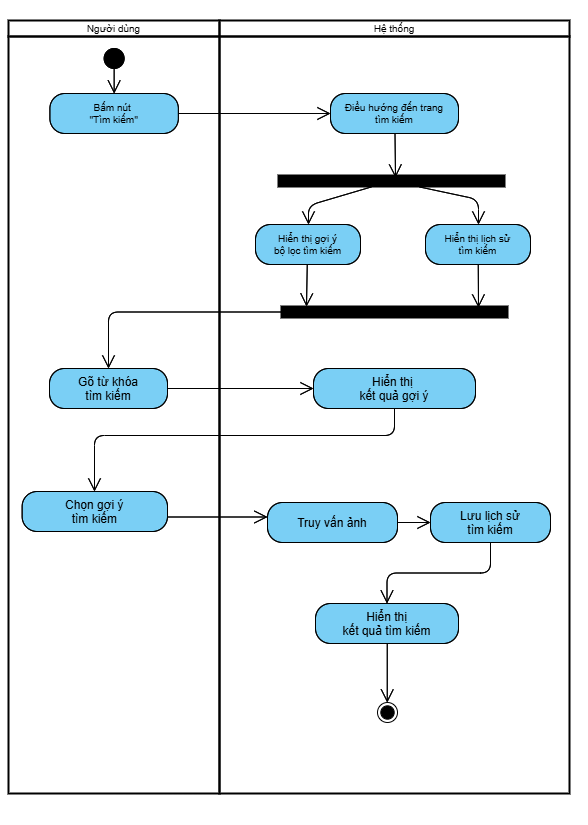
\includegraphics[width=0.6\linewidth]{figures/c3/3-3-16-activity-diagram.png} 
    &  
    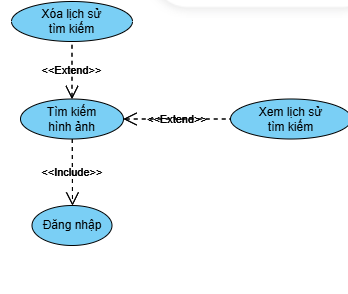
\includegraphics[width=0.35\linewidth]{figures/c3/3-3-16-relationship.png} \\ 
    \hline
\end{tabular}
\end{table}

\begin{figure}[H]
    \centering  
    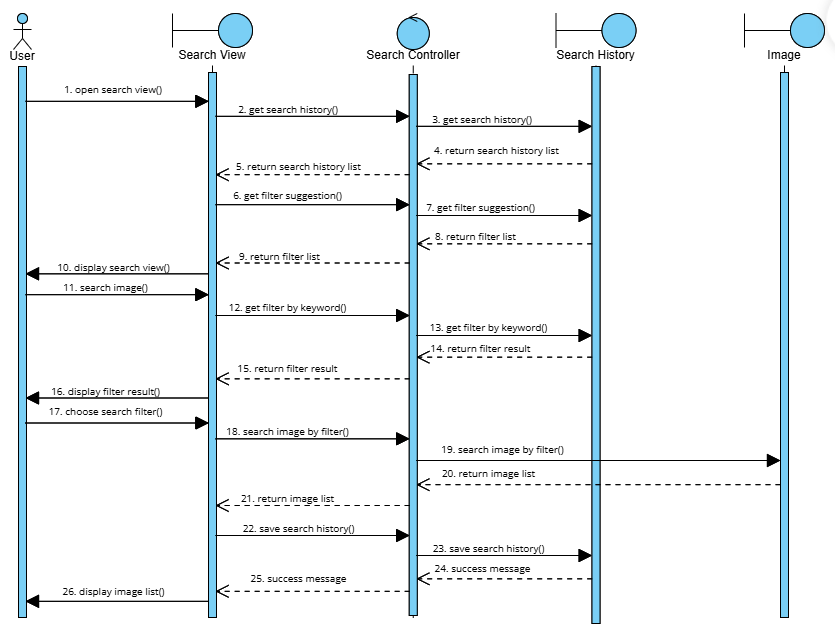
\includegraphics[width=1.1\textwidth]{figures/c3/3-3-16-sequence-diagram.png}
    \caption{Biểu đồ tuần tự ca sử dụng tìm kiếm hình ảnh.}
    \label{fig:3-3-16-sequence-diagram}
\end{figure}